\documentclass{beamer}
\usepackage[utf8]{inputenc}

\usetheme{Madrid}
\usecolortheme{default}
\usepackage{amsmath,amssymb,amsfonts,amsthm}
\usepackage{txfonts}
\usepackage{tkz-euclide}
\usepackage{listings}
\usepackage{adjustbox}
\usepackage{array}
\usepackage{tabularx}
\usepackage{gvv}
\usepackage{multicol}   % <-- Add this

\usepackage{enumitem}
\setlist{nosep}              % optional spacing tweak
\setlist[enumerate]{label=\arabic*.}  % optional numbering tweak
\makeatletter

\let\beamer@enum@patch\relax
\makeatother
\usepackage{lmodern}
\usepackage{circuitikz}
\usepackage{tikz}
\usepackage{graphicx}
\usepackage{mathtools}
\setbeamertemplate{page number in head/foot}[totalframenumber]

\usepackage{tcolorbox}
\tcbuselibrary{minted,breakable,xparse,skins}



\definecolor{bg}{gray}{0.95}
\DeclareTCBListing{mintedbox}{O{}m!O{}}{%
  breakable=true,
  listing engine=minted,
  listing only,
  minted language=#2,
  minted style=default,
  minted options={%
    linenos,
    gobble=0,
    breaklines=true,
    breakafter=,,
    fontsize=\small,
    numbersep=8pt,
    #1},
  boxsep=0pt,
  left skip=0pt,
  right skip=0pt,
  left=25pt,
  right=0pt,
  top=3pt,
  bottom=3pt,
  arc=5pt,
  leftrule=0pt,
  rightrule=0pt,
  bottomrule=2pt,
  toprule=2pt,
  colback=bg,
  colframe=orange!70,
  enhanced,
  overlay={%
    \begin{tcbclipinterior}
    \fill[orange!20!white] (frame.south west) rectangle ([xshift=20pt]frame.north west);
    \end{tcbclipinterior}},
  #3,
}
\lstset{
    language=C,
    basicstyle=\ttfamily\small,
    keywordstyle=\color{blue},
    stringstyle=\color{orange},
    commentstyle=\color{green!60!black},
    numbers=left,
    numberstyle=\tiny\color{gray},
    breaklines=true,
    showstringspaces=false,
}


\title 
{12.296}
\date{November 3, 2025}


\author 
{Dhanush Kumar A - AI25BTECH11010}



\begin{document}
\frame{\titlepage}
\begin{frame}{Question}


The area enclosed between the straight line $y = x$ and the parabola $y = x^2$ in the $xy$-plane is (PI 2012)

\begin{multicols}{2}
\begin{enumerate}
\item $\dfrac{1}{6}$
\item $\dfrac{1}{4}$
\item $\dfrac{1}{3}$
\item $\dfrac{1}{2}$
\end{enumerate}
\end{multicols}
\end{frame}
\begin{frame}{Solution}
For $y = x^2$, we write it in matrix form as
\begin{align}
\vec{x}^{\top} V \vec{x} + 2\vec{u}^{\top}\vec{x} + f = 0
\end{align}
where
\begin{align}
V = \myvec{1 & 0 \\ 0 & 0}, \quad 
\vec{u} = \myvec{0 \\ -\tfrac{1}{2}}, \quad 
f = 0.
\end{align}

The line $y = x$ can be written parametrically as
\begin{align}
\vec{x} = \vec{h} + \kappa \vec{m}, \quad \kappa \in \mathbb{R}
\end{align}
where
\begin{align}
\vec{h} = \myvec{0 \\ 0}, \quad 
\vec{m} = \myvec{1 \\ 1}.
\end{align}

The intersection points satisfy
\begin{align}
\kappa_i =
\frac{-\vec{m}^{\top}(V\vec{h} + \vec{u}) 
\pm \sqrt{[\vec{m}^{\top}(V\vec{h} + \vec{u})]^2 
- (\vec{m}^{\top}V\vec{m})\,g(\vec{h})}}
{\vec{m}^{\top}V\vec{m}}
\end{align}
\end{frame}
\begin{frame}{Solution}

where
\begin{align}
g(\vec{h}) = \vec{h}^{\top}V\vec{h} + 2\vec{u}^{\top}\vec{h} + f.
\end{align}

Substituting values:
\begin{align}
V\vec{h} + \vec{u} &= \myvec{0 \\ -\tfrac{1}{2}}, \\
\vec{m}^{\top}(V\vec{h} + \vec{u}) &= -\tfrac{1}{2}, \\
\vec{m}^{\top}V\vec{m} &= 1, \\
g(\vec{h}) &= 0.
\end{align}

Hence,
\begin{align}
\kappa_{1,2} &= 
\frac{-(-\tfrac{1}{2}) \pm \sqrt{(-\tfrac{1}{2})^2 - 1(0)}}{1} \\
&= \frac{\tfrac{1}{2} \pm \tfrac{1}{2}}{1}.
\end{align}
\end{frame}
\begin{frame}{Solution}

Therefore,
\begin{align}
\kappa_1 = 0, \quad \kappa_2 = 1.
\end{align}

The intersection points are
\begin{align}
\vec{x}_1 = \vec{h} + \kappa_1 \vec{m} = \myvec{0 \\ 0}, \quad
\vec{x}_2 = \vec{h} + \kappa_2 \vec{m} = \myvec{1 \\ 1}.
\end{align}
\end{frame}
\begin{frame}{Solution}

The area enclosed between the line and the parabola is
\begin{align}
A &= \int_{0}^{1} (y_{\text{line}} - y_{\text{parabola}})\,dx \\
  &= \int_{0}^{1} (x - x^2)\,dx \\
  &= \left[\frac{x^2}{2} - \frac{x^3}{3}\right]_0^1 \\
  &= \frac{1}{2} - \frac{1}{3} \\
  &= \frac{1}{6}.
\end{align}
\end{frame}
\begin{frame}{Solution}

\begin{align}
\boxed{A = \frac{1}{6}}
\end{align}

\noindent\textbf{Final Answer: (a) } $\dfrac{1}{6}$



\end{frame}
\begin{frame}{Plot}
    \centering
    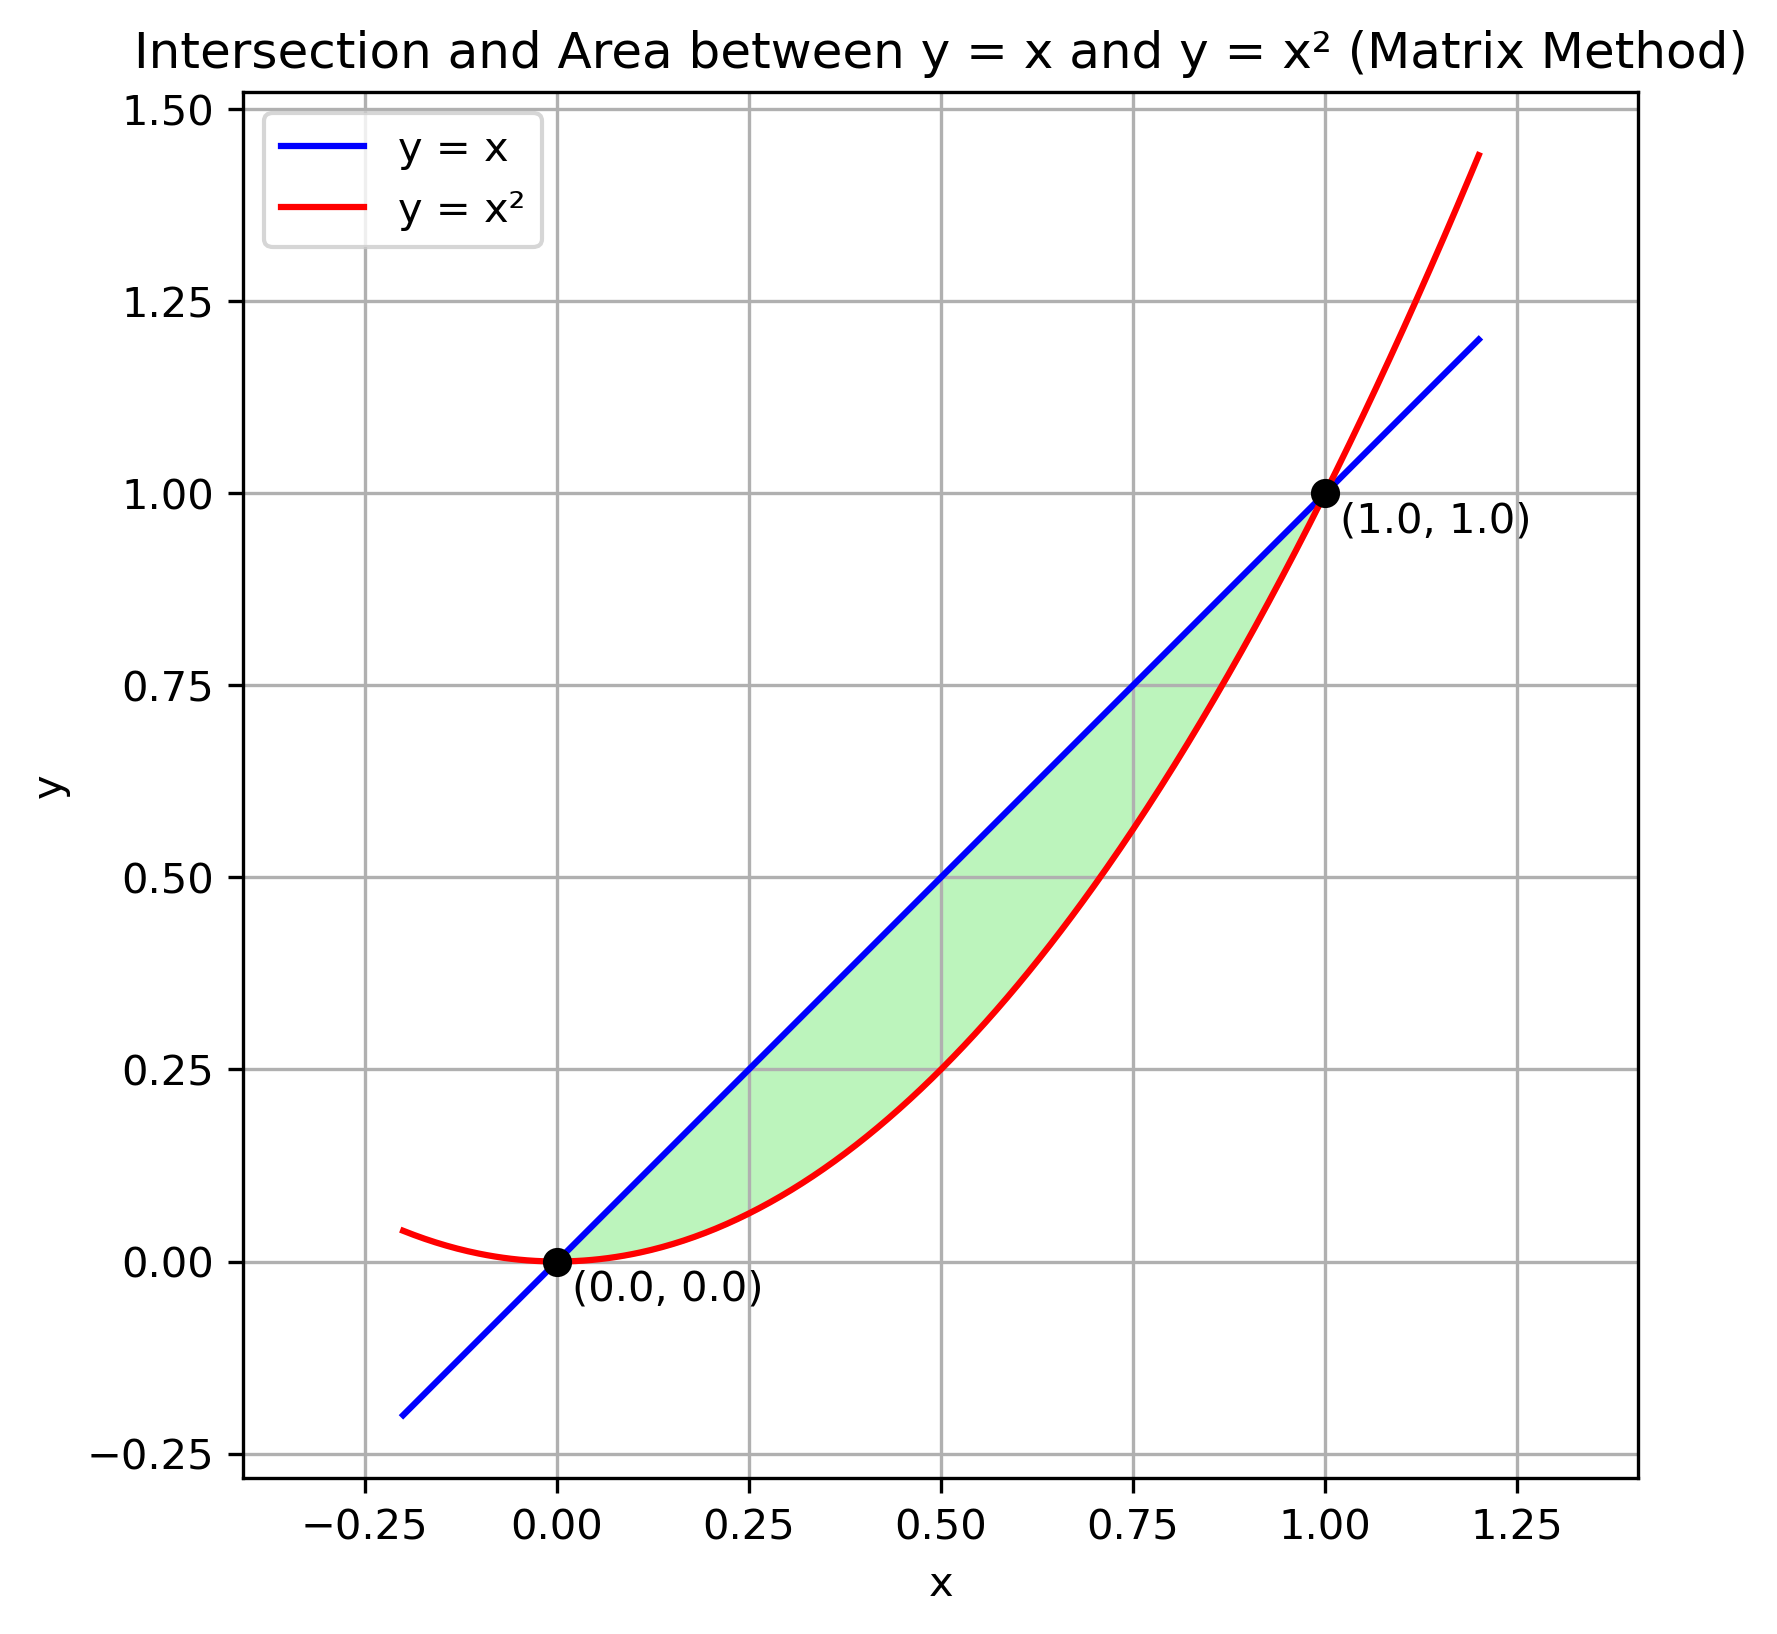
\includegraphics[width=\columnwidth, height=0.8\textheight, keepaspectratio]{../figs/matrix_intersection_area.png}     
\end{frame}

\end{document}



